% vim: set tw=78 sts=2 sw=2 ts=8 aw et ai:

In order to explain the algorithms used for determining historical relevance, let's first analyze a typical time series, using as example a word that carries a heavy influence on history: war.

\begin{figure*}[ht]
\centering
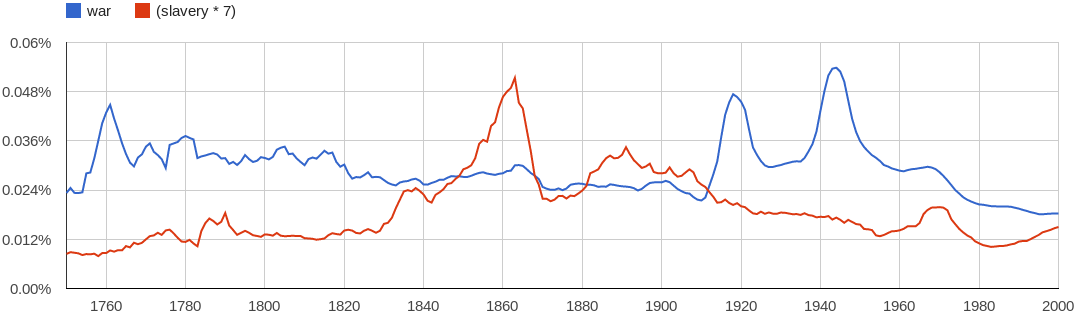
\includegraphics[max size={0.7 \textwidth}{0.7 \textheight}]{war-series}
\caption{Ngram time series for war and slavery}
\label{fig:war-series}
\end{figure*}

Taking a look at Figure~\ref{fig:war-series}, the first feature of the plot that can be noticed is the presence of several well-defined peaks, corresponding to the following historic events: Seven Years' War ($1755 - 1765$), World War I ($1910 - 1926$) and World War II ($1936 - 1953$). A closer inspection reveals further peak-like shapes, some of which can be identified with major wars in history: American Revolutionary War ($1775 - 1783$), American Civil War ($1860 - 1871$) and Vietnam War ($1961 - 1978$). One must note that the shape of a singular plot can only reveal so much information, but by determining historical relevance for different n-grams and correlating the results, one can viably get a picture of a historic event.

The remainder of this section shall focus on algorithms for peak detection. The main requirement for such an algorithm is the capability of quantitatively measuring the historical relevance of that peak. For example, the three large peaks of the n-gram war should be assigned a high historical relevance. Note that the value of the historical relevance needs not be constant over the entire peak.

\subsubsection{Double Change Peak Detection}

Instead of performing full peak detection, it is simpler to find the portions of abrupt increase and decrease that form a peak. Formally, we say that a time series $\left\{ s_{i, t} \right\}$ suffers a double increase or decrease if it increases or decrease twice consecutively. Furthermore, the magnitude of that increase (Equation~\ref{eq:double-increase}) or decrease (Equation~\ref{eq:double-decrease}) at time $t$ is defined as the maximum $x \in \left[ 0, 1 \right]$ that satisfies one of the following equations:

\begin{align}
\label{eq:double-increase}
s_{i, t} > \left( 1 + x \right) s_{i, t - 1}, \, s_{i, t + 1} > \left( 1 + x \right) s_{i, t}
\\
\label{eq:double-decrease}
s_{i, t} < \left( 1 - x \right) s_{i, t - 1}, \, s_{i, t + 1} < \left( 1 - x \right) s_{i, t}
\end{align}

Furthermore, the magnitude of a single increase (Equation~\ref{eq:single-increase}) or of a single decrease (Equation~\ref{eq:single-decrease}) at time $t$ is defined as the maximum $x \in \left[ 0, 1 \right]$ that satisfies one of:

\begin{align}
\label{eq:single-increase}
s_{i, t} &> \left( 1 + 2x \right) s_{i, t - 1}
\\
\label{eq:single-decrease}
s_{i, t} &< \left( 1 - 2x \right) s_{i, t - 1}
\end{align}

The magnitude $m_{i, t}$ of the change around a point $t$ is defined as the maximum between the magnitude of the double change and the magnitude of the single change at that point. We then define the historical relevance $r_{i, t} = \min \left( \left\lfloor 10 m_{i, t} \right\rfloor, 9 \right)$.

\subsubsection{Linear Model Peak Detection}

Generalizing the previous idea, one can use a linear model for approximating portions of the time series. The core of this approach is to fit lines to the graph of the time series using linear regression, by considering larger and larger intervals until the error rises above a given threshold. Of course, the series must initially be normalized by using the standard score.

Thus, upon finding a maximal interval fitted by a line within a small error, the magnitude of the change on that interval is defined as a linear function of the logarithm of the slope. This choice is motivated by the wide range of values that the slope can take, forming a sort of heavy-tailed distribution. The historical relevance on that interval is computed as follows: $r_{i, t} = \max \left( \left\lfloor m_{i, t} \right\rfloor, 0 \right)$.

\subsubsection{Gaussian Model Peak Detection}

Another completely different idea for peak detection is to notice that peaks are usually shaped like a Gaussian distribution. Let us consider a time interval $\left[ l, r \right] \subseteq \left[ 1500, 2008 \right]$ and the time series for some word $w_i$ on that interval, $\left\{ s_{i, t} \right\}_{t=l}^{r}$. Initially, one must normalize the series to get a probability distribution:

\begin{align}
\label{eq:gaussian-normalization}
g_{i, t} &= \frac{s_{i, t} - \min_{p \in \overline{l, r}} s_{i, p}}{\sum_{q = l}^{r} \left( s_{i, q} - \min_{p \in \overline{l, r}} s_{i, p} \right)}.
\end{align}

This is approximated by a normal distribution $N \left( \mu, \sigma \right)$ with the following parameters:

\begin{align}
\label{eq:mu-gaussian-model}
\mu &= \sum_{t=l}^{r} g_{i, t} t, \\
\label{eq:sigma-gaussian-model}
\sigma^2 &= \sum_{t=l}^{r} g_{i, t} \left( t - \mu \right)^2.
\end{align}

The similarity between $g_{i, t}$ and $N \left( \mu, \sigma \right)$ is computed using the earth mover's distance introduced in \newcite{rubner98metric}. Unfortunately, we have to consider all possible intervals $\left[ l, r \right] \subseteq \left[ 1500, 2008 \right]$, which leads to cubic complexity. This can be improved by using a heuristic to decide if a probability distribution even remotely looks like a Gaussian bell. As evidenced in \newcite{balanda88kurtosis}, one such measure is kurtosis, which is defined in terms of the fourth moment about the mean $\mu_4$: $\gamma_2 = \frac{\mu_4}{\sigma^4} - 3$. Kurtosis can be computed in constant time for any interval, using trivial preprocessing of partial sums, so we are able to efficiently determine intervals on which the kurtosis is sufficiently close to $0$.

Next, we sort the remaining intervals in increasing order of the earth mover's distance to the Gaussian, imposing a limit of $0.3$ on that value, and process them. Intervals that intersect previously processed ones are simply ignored, which both ensures that the intervals are disjoint and that only the highest quality peaks are chosen.

Finally, we compute the magnitude of the change on an interval $\left[ l, r \right]$ as the percentage with which the Gaussian peak increases from its smallest value to its largest value:

\begin{align}
\label{eq:gaussian-magnitude}
m_i \left( \left[ l, r \right] \right) &= \frac{N \left( \mu, \sigma \right) \left( \mu \right) \cdot \sum_{q} \left( s_{i, q} - \min_{p} s_{i, p} \right)}{\min_{p} s_{i, p}}.
\end{align}

One way to define historical relevance in this case is to assign it a constant value on the interval: $r_{i, t} = \left\lfloor 10 \cdot \min \left( m_i \left( \left[ l, r \right] \right), 1) \right) \right\rfloor$.

An alternative way is to assign variable relevance, such that it also forms a Gaussian bell. The formula, that also includes a widening parameter $w \in \left[ 1, \infty \right)$, is as follows:

\begin{align}
\label{eq:gaussian-model-variable-relevance}
r_{i, t} \left( w \right) &= r_{i, t} \cdot \frac{N \left( \mu, w \sigma \right) \left( t \right)}{N \left( \mu, w \sigma \right) \left( \mu \right)}, \, \forall t \in \left[ l, r \right].
\end{align}

\subsubsection{Graphical Analysis}

\begin{figure}[t]
\centering
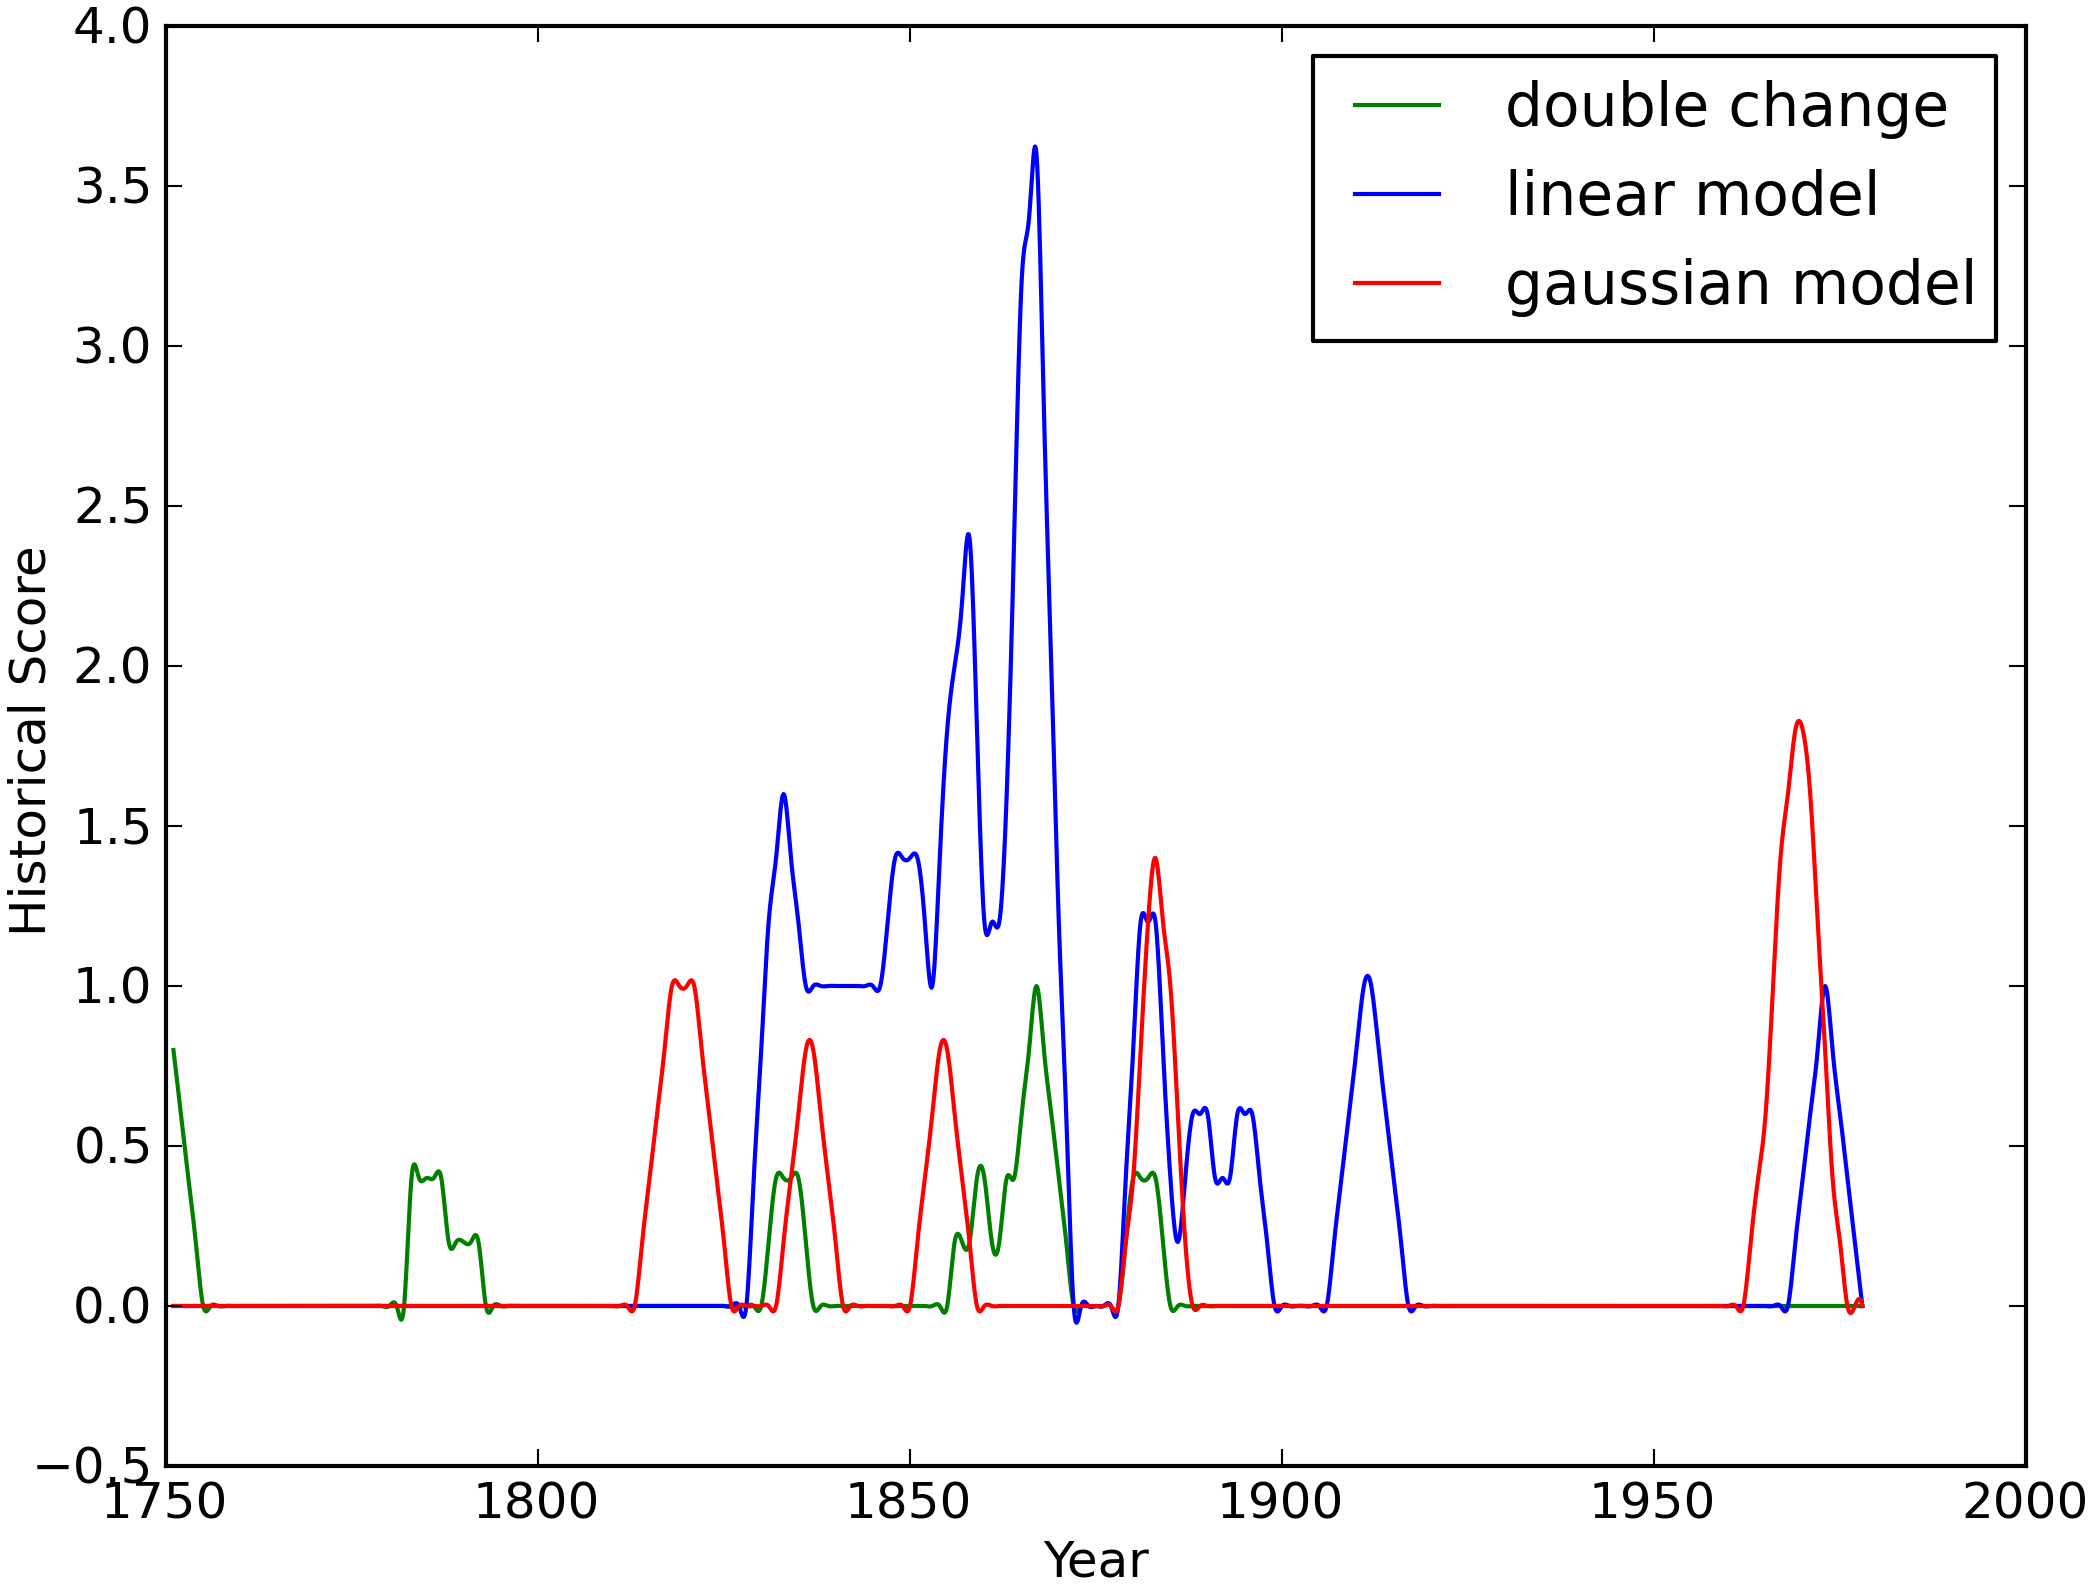
\includegraphics[max size={0.5 \textwidth}{0.5 \textheight}]{slavery-relevance}
\caption{Historical relevance of slavery}
\label{fig:slavery-relevance}
\end{figure}

Of the three algorithms, it cannot be said that one of the them performs the best at detecting and characterizing peaks. However, with the help of an example such as Figure~\ref{fig:slavery-relevance}, one can point the strengths and weaknesses of each of them (for the Gaussian model, the widening parameter used is $w = 2$). As can be seen in Figure~\ref{fig:war-series}, slavery has had two important "historic peaks": the first, between $1842$ and $1871$, includes the American Civil War, while the second, between $1964$ and $1979$, includes the African-American Civil Rights Movement.

The first peak is detected by all three algorithms. The best detection is performed by the linear model, since it can be approximated well by 2 lines. The other algorithms also detect activity in this period, but in 2 distinct intervals. Notably, the second interval detected by the Gaussian model is centered around the American Civil War. The conclusion is that although the linear model is better at detecting triangular peaks, the Gaussian model does a better job at identifying the high point that probably corresponds to a historic event. The double change model is significantly worse than the other two, since it assigns more relevance to the tails of the triangle.

The second peak is detected only by the last two algorithms. Although both reasonably identify the peak, the Gaussian model performs better by considering a slightly larger interval. This is to be expected, as the peak is roughly bell-shaped.

Lastly, the double change model also detects a minor peak centered around $1790$. In that period, the Constitution of the United States was drafted, and one if its highlights was the Three-Fifths Compromise, which stated that for representation purposes, slaves counted as only three-fifths of a person. Thus, although theoretically inferior to the other two algorithms, the double change model has the capability of detecting less important historic events.
